% ----------------------Adding the necessary packages------------------------------
% We need to specify the document type and the encoding first
\documentclass[12pt]{article}
\usepackage[utf8]{inputenc}

% defining margin for the document
\usepackage[margin=1in]{geometry}

% use these packages for tables
\usepackage{booktabs}
\usepackage{tabu}

% use for making captions beautiful
\usepackage[labelfont=bf, skip=5pt, font=small]{caption}

% these packages are used for images
\usepackage{graphicx}

% package for color
\usepackage{xcolor}

% position images precisely at location in text
\usepackage{float}



% ----------------------Rules to follow document wide------------------------------
% keep 1em space between blank lines
\setlength{\parskip}{1em}
% don't indent new paragraphs
\setlength{\parindent}{0em}


% ----------------------We enter our text here--------------------------------------
%-----------------------------------------------------------------------------------
\begin{document}

%------------------------ The document title and authors-----------------------------
\begin{center}
    % largest text
    \huge{Our project title}
    
    % "\\" stands for newline and 10pt for the space between the lines
    \\[10pt]
    
    % large text
    \large{The authors}
\end{center}
\rule{\textwidth}{0.5pt}

%-----------------------Introduction to our functions-------------------------------
\section{Introduction to the functions}

%-----------------------Arnab's part------------------------------------------------
\subsection{The tangent function}
    The tangent function is one of the six trigonometric functions. It has many important uses in real life calculations such as calculating the slope of straight lines, angles of elevation and depression \cite{tanexamplewebsite1}, rate of altitude change of an aircraft \cite{tanexamplewebsite2} etc. \\
    The tangent function can be understood from an unit circle(a circle whose radius = 1).
    % inserting image of unit circle
    \begin{figure} [!h]
        \centering
        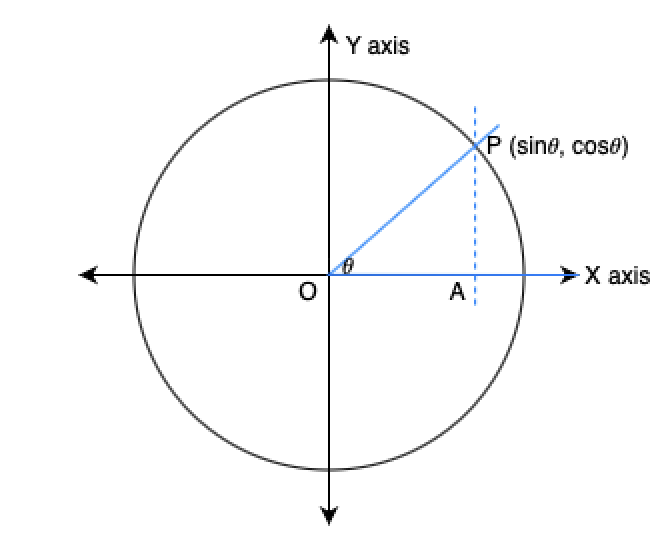
\includegraphics[width=0.4\textwidth]{Unit-circle.png}
        \caption{A unit circle}
        % labels help us to refer to within text and doesn't have any visual impact
        \label{fig:unit_circle}
    \end{figure} \\
    In a unit circle we take two lines originating from the center, one along the positive x axis and the other line intersecting the circumference of the circle. From the definition of unit circle, the coordinate of the point at which the circumference is intersected is $(\sin\theta, \cos\theta)$ \cite{unitcirclewebsite} and the tangent of the angle $\theta$ is:
    \begin{equation}
        \tan(\theta) = \sin(\theta) \div \cos(\theta) \label{tan_formula_1}
    \end{equation}
    The domain of $\tan \theta$ is x $\in \mathbb{R}$, x $\ne$ ($\pi$/2) + n*$\pi$ and its codomain is (-$\infty$, $\infty$) \cite{tandomainwebsite}.
    % inserting image of tangent graph
    \begin{figure} [H]
        \centering
        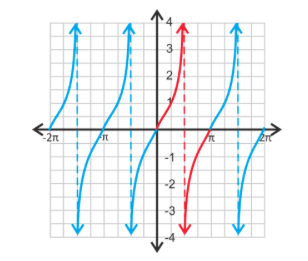
\includegraphics[width=0.4\textwidth]{graph-of-tangent.png}
        \caption{Graph of tangent function}
        % labels help us to refer to within text and doesn't have any visual impact
        \label{fig:graph_tangent}
    \end{figure} 
    The graph of the tangent function has some interesting properties. As cos$\theta$ = 0 when $\theta$ = $\pm$(n$\pi$/2) where n is odd, the graph approaches an asymptote along y-axis as cos$\theta$ approaches 0. Moreover, the graph has no amplitude and the period is calculated as the distance between any two high points or low points at the same height and the period is $\pi$. The graph intersects the y-axis only at (0,0) and the x-axis for $\theta$ = n$\pi$.
    
    \bibliographystyle{ieeetr}
    \bibliography{bibliography}
\end{document}
